\setchapterstyle{kao}
\setchapterpreamble[u]{\margintoc}
\chapter{Digital interfaces for environmental sensors}
\labch{digital_interfaces}

In \refch{circuits_intro}, we considered the fundamentals of constructing circuits that exploit the abilities of microcontrollers to measure voltage and time to quantify environmental variables.
These circuits were based on \textit{analog} sensors -- that is, sensors that return signals in the form of continuously variable voltages or time lags.
By integrating the microcontroller, circuit and analog sensor components, you assembled a device that provided a \textit{digital} signal -- a number that represents an observation of the corresponding environmental parameter.

A modern trend in sensor development is \textit{digital sensors}, whose output is intrinsically in the form of numbers rather than voltage or time.
If you used the external \DS3231 Real Time Clock in \refch{time_keeping}, you have already used a digital sensor.
In digital sensors, the circuitry and some of the microcontroller functions that you used to convert analog signals to digital outputs have been placed on the sensor itself.
This means that the user-designed circuitry and microcontroller interfaces can usually be greatly simplified compared to an analog sensor measuring the same quantity.

Because digital sensors typically return observations as numbers with many decimal places, it's tempting to overlook the fact that in many cases they may be less accurate and precise than analog sensors (or may cost more for comparable accuracy and precision).
It's important to keep in mind that digital sensors have the same basic operating principles and limitations as analog sensors.
The internal circuitry of digital sensors is designed by experts and mass-produced in sophisticated factories.
This means that the tradeoffs and optimizations in sensitivity, resolution, power consumption, \etc that you considered in working with analog sensors have been decided by highly skilled professionals.
Remember, though, that these circuits (and hence the digital sensors that use them) still have most of the same constraints you wrestled with in your own sensor design.

With those caveats in mind, digital sensors often have a number of advantages relative to analog sensors.
Depending on the type of digital sensor and the context, these advantages may include:
\begin{itemize}
	\item Digital sensors use digital \texttt{GPIO}s, which are more abundant than analog \texttt{GPIO}s on most microcontrollers;
	\item Protocols for communicating with digital sensors are two-way -- information such as settings, commands to take readings \etc can be sent to digital sensors to make them more efficient and versatile;
	\item Some digital sensor protocols support multiple sensors on one set of \texttt{GPIO}s and wires, with microcontrollers able to identify and query each of those sensors individually;
	\item Some digital protocols support very long wire connections (though others are limited to very short wires);
	\item Some digital sensors internally do complex computations, such as integrating angular orientation from angular accelerations, which would be expensive in terms of processor cycles and energy to perform on a microcontroller.
\end{itemize}
These advantages are evident in many industrial applications (cars, phones, \etc).
As a result, many useful digital environmental sensors are mass produced and amazingly cheap for their capabilities.

This chapter uses examples of readily available and scientifically informative environmental sensors to illustrate how to use several common communication protocols for digital sensors.
Many other examples using each of these protocols appear later in this book, in applications of data from digital sensors to drawing inferences and hypothesis testing about environmental mechanisms.
For some readers, one or two of these protocols may be sufficient for the examples and data collection applications at hand.
If so, it may be an efficient strategy to focus on that subset of protocols, returning to learn the others if and when the need arises.

\subsection{Communicating with digital sensors}
In practice, getting measurements from digital sensors usually involves two main elements: establishing the appropriate circuit connections, and finding (or, occasionally, writing) a \emph{driver}.
A driver is a piece of code that interfaces between a microcontroller and digital sensor.
The driver enables the user to interact with a digital sensor, \eg by setting measurement parameters or querying for data, with simple, intuitive high-level \Micropython commands.
The driver handles messages between the microcontroller and the digital sensor at a very low level, that takes some technical expertise and patience to understand.
Fortunately, \Micropython-based drivers are freely available online for many of the most useful digital environmental sensors, and more are being written all the time.
You typically don't need to know much about the inner workings of a driver to use it for obtaining environmental sensor readings.

Most digital sensors used in environmental sensing communicate using one of four protocols:

%\begin{itemize}
%	\item \textbf{Inter-Integrated Circuit (\i2c)}
%
%	The \htmladdnormallink{\i2c}{https://en.wikipedia.org/wiki/I\%C2\%B2C} protocol (pronounced ``eye squared sea'') is commonly used in digital sensors for time, light, accceleration, \etc, and is also used in many small TFT displays for microcontrollers.
%	%Adafruit provides a useful \htmladdnormallink{overview of \i2c}{https://learn.adafruit.com/adafruit-ft232h-with-spi-and-i2c-libraries/i2c-devices}.
%	\i2c is a ``2 wire'' protocol (in addition to \texttt{Vin} and \texttt{GND}).
%	\i2c is designed to work over relatively short distances ($\le$ a few meters), but \htmladdnormallink{\texttt{differential extenders}}{https://learn.sparkfun.com/tutorials/qwiic-differential-i2c-bus-extender-pca9615-hookup-guide/all} are available that greatly increase the distance over which \i2c devices can communicate.
%
%	\smallskip
%	\i2c supports multiple devices on one cable, but each device must have unique addresses.
%	Adafruit has written a useful \htmladdnormallink{summary of default \i2c addresses}{https://cdn-learn.adafruit.com/downloads/pdf/i2c-addresses.pdf}, describing addresses used by different types of sensors and other devices.
%	Because there are more types of devices than distinct addresses, there is overlap between the addresses of some different sensor types.
%	It's largely a matter of luck whether two sensor types have conflicting addresses, but works out most of the time.
%	Some \i2c devices have a mechanism, like movable jumpers, to change \i2c addresses so that two or more of these devices can co-exist on the same cable.
%
%	\item \textbf{1-Wire}
%
%	\htmladdnormallink{1-wire}{https://en.wikipedia.org/wiki/1-Wire} is a proprietary protocol design that, as the name implies, uses only one wire in addition to \texttt{Vin} and \texttt{GND}.
%	1-wire is used in relatively few sensor types, but is worth knowing about because one of those is an inexpensive and versatile \htmladdnormallink{temperature sensor}{https://datasheets.maximintegrated.com/en/ds/DS18B20.pdf} that is among the most useful available for environmental monitoring.
%
%	\smallskip
%	1-wire supports many (up to hundreds) of devices on a single cable, each of which can be independently queried for sensor readings because it has a unique ROM address.
%	1-wire supports lower (but still generally sufficient) data rates than \i2c, which (when properly configured) can operate over much longer cables.
%
%	\item \textbf{Universal Asynchronous Receiver-Transmitter (\uart)}
%
%	\htmladdnormallink{\uart}{https://en.wikipedia.org/wiki/Universal_asynchronous_receiver-transmitter} is a communications protocol with a long history of use in computer hardware (including communication between computers and microcontrollers), navigation equipment and many other industrial applications.
%	\uart supports communication between only two devices, and these devices must share common settings for a number of parameters. %(bit speed, character length, parity, and stop bits).
%	Common applications in environmental sensing include \texttt{GPS} receivers and Air Quality Index sensors.
%
%	\uart uses two wires (in addition to \texttt{Vin} and \texttt{GND}), one for transmitting and one for receiving.
%	In some applications (\eg, some \texttt{GPS} configurations) only one of these functions is utilized (\eg, transmit on the \texttt{GPS} and receive on the microcontroller) in which case only one of these wires is necessary.
%
%	\item \textbf{Serial Peripheral Interface (\spi)}
%
%	The \spi protocol is commonly used for some types of sensors, external radio communications, TFT displays, LED banks, \etc
%	\spi uses four wires (in addition to \texttt{Vin} and \texttt{GND}), three of which can be shared by multiple devices on the same cable but the fourth of which must be unique to each device.
%	Maximum data rates are higher than for \i2c devices.
%	Many digital sensors have both \spi and \i2c interfaces, so they can be used with either protocol.
%
%	%►Overview: https://learn.sparkfun.com/tutorials/serial-peripheral-interface-spi
%	%Technical info: https://en.wikipedia.org/wiki/Serial\_Peripheral\_Interface\_Bus
%	%Also see Adafruit tutorials on SPI sensors
%\end{itemize}

\begin{itemize}
	\item \textbf{Inter-Integrated Circuit (\i2c)}

	The \htmladdnormallink{\i2c}{https://en.wikipedia.org/wiki/I\%C2\%B2C} protocol (pronounced ``eye squared sea'') is commonly used in digital sensors for time, light, accceleration, \etc, and is also used in many small TFT displays for microcontrollers.

	\item \textbf{1-Wire}

	\htmladdnormallink{1-wire}{https://en.wikipedia.org/wiki/1-Wire}  is used in relatively few sensor types, but is worth knowing about because one of those is an inexpensive and versatile \htmladdnormallink{temperature sensor}{https://datasheets.maximintegrated.com/en/ds/DS18B20.pdf} that is among the most useful available for environmental monitoring.


	\item \textbf{Universal Asynchronous Receiver-Transmitter (\uart)}

	\htmladdnormallink{\uart}{https://en.wikipedia.org/wiki/Universal_asynchronous_receiver-transmitter} is a communications protocol with a long history of use in computer hardware, including communication between computers and microcontrollers.
	\uart is used in many Global Positioning System (GPS) receivers and Air Quality Index (AQI) sensors, in some Automatic Identification System (AIS) navigation equipment, and many other industrial applications.

	\item \textbf{Serial Peripheral Interface (\spi)}

	The \htmladdnormallink{\spi}{https://learn.sparkfun.com/tutorials/serial-peripheral-interface-spi} protocol is commonly used for some types of sensors, external radio communications, TFT displays, LED banks, \etc \spi interfaces are used on some microcontrollers to read from and write to microSD cards.
\end{itemize}



\section{\color{gray}\i2c sensors \color{black}}
\labsec{i2c_sensors}
\subsection{Background}
	%Adafruit provides a useful \htmladdnormallink{overview of \i2c}{https://learn.adafruit.com/adafruit-ft232h-with-spi-and-i2c-libraries/i2c-devices}.
\i2c is a ``2 wire'' protocol: it has two communications connections, \texttt{SDA} and \texttt{SCL}, in addition to \texttt{Vin} and \texttt{GND}.
Most microcontrollers have built-in hardware  \texttt{GPIO}s preconfigured as \texttt{SDA} and \texttt{SCL} for \i2c communications.
On most microcontrollers, it is also possible to use other \texttt{GPIO} pins for software-driven \i2c communications (``bit-banging''), often with somewhat reduced but perfectly adequate capabilities.
%This provides helpful flexibility when preconfigured \texttt{SDA} and \texttt{SCL} \texttt{GPIO}s are need for other uses, or when too many \i2c devices are needed .

\i2c is designed to work over relatively short distances ($\le$ a few meters), but \htmladdnormallink{\texttt{differential extenders}}{https://learn.sparkfun.com/tutorials/qwiic-differential-i2c-bus-extender-pca9615-hookup-guide/all} are available that greatly increase the distance over which \i2c devices can communicate.

A useful feature of \i2c is that it supports multiple devices on one cable (here, we're using ``cable'' as shorthand for the \i2c bus on the microcontroller, the wires connecting the microcontroller to the sensors, \etc).
However, there is a constraint: each device must have an address that is unique on any given cable.

Each type of \i2c-based digital sensor is typically pre-programmed with an address, associated with what kind of sensor it is.
This is very helpful for authors of \emph{drivers} (short codes designed to interface between a microcontroller and digital sensor).
However, it means that trying to use multiple sensors of the same type on a single \i2c cable often runs afoul of the unique address constraint.

Because there are more types of devices than distinct addresses, there are also overlaps between the addresses of some different sensor types.
Adafruit has written a useful \htmladdnormallink{summary of default \i2c addresses}{https://cdn-learn.adafruit.com/downloads/pdf/i2c-addresses.pdf}, describing addresses used by different types of sensors and other devices.


It's largely a matter of luck whether two sensor types have conflicting addresses, but works out most of the time.

For cases when it doesn't, some \i2c devices have a mechanism, like movable jumpers, to change \i2c addresses so that two or more of these devices can co-exist on the same cable.
Another alternative, of course, is to have more than one \i2c bus, \eg by having separate hardware and bit-banged \i2c buses.
Still another workaround is an \i2c \htmladdnormallink{multiplexer}{https://github.com/mcauser/micropython-tca9548a}, which is an \i2c device that can direct communications to any of eight \i2c devices attached to it (whether or  not they have the same addresses).
% The reference to the external RTC is \refsec{ext_i2c_time}

\subsection{\color{gray} Measuring temperature with a high-resolution sensor \color{black}}

\subsubsection{\howto Set up an \MCP9808 temperature sensor}

\begin{marginfigure}
	\begin{center}
		\htmladdnormallink{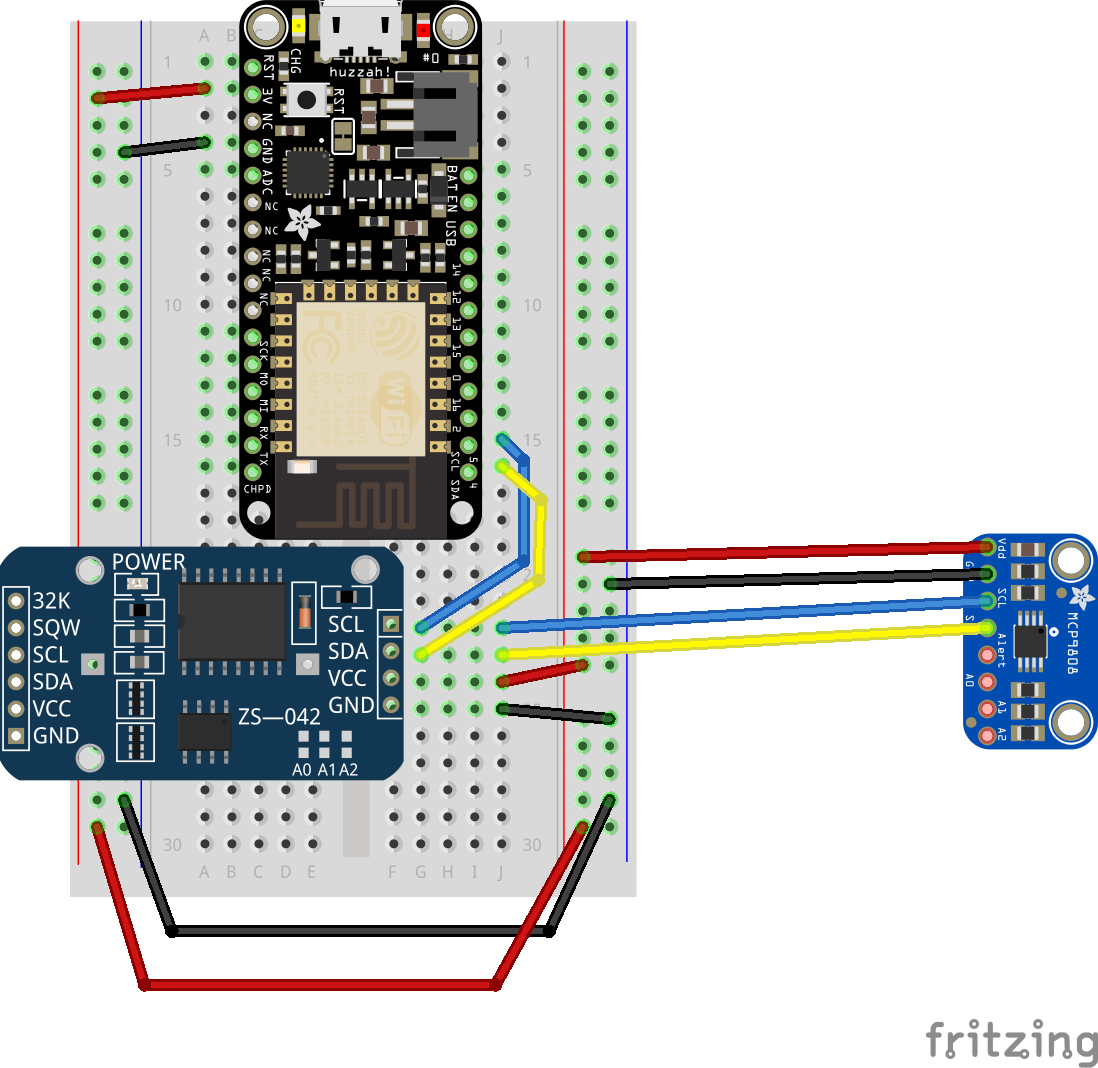
\includegraphics[width=\MFW]{Fritzing/feather_MCP9808_bb.png}}{https://github.com/publicsensors/IntroSensors/blob/digital/Fritzing/feather_MCP9808_bb.png}
		%\includegraphics[height=5cm]{Images/DS3231breadboard.jpg}
		\caption[MCP9808 on breadboard]{An example of layout and wire connections for the \MCP9808 temperature sensor and ESP8266 microcontroller. The circuit layout is similar to that used for the DS3231 external Real Time Clock. The DS3231 is left in the figure to emphasize that \i2c can support multiple devices simultaneously, but this exercise works equally well with or without the DS3231.}
		\labfig{mcp9808_breadboard}
	\end{center}
\end{marginfigure}


The circuit layout for the \MCP9808 is shown in \reffig{mcp9808_breadboard}.

https://github.com/kfricke/micropython-mcp9808

\begin{enumerate}
	\item This is a test of the glossary: \gls{ssw_connector}. \Gls{ssw_connector}, too.
	\item This is a test of the glossary: \gls{computer}.

	\item \textbf{Connect the GND and 3V pins on the ESP8266 to the GND and Vdd pins on the \MCP9808}.

	Like in the thermistor calibration in \refsec{cal_therm}, we will use ``water baths'' made of paper cups to expose the \MCP9808 sensors to known temperatures without getting them wet.
	This is most easily done if the sensor is connected to the microcontroller by extra long wires.
	If your \MCP9808 has pins soldered to it, you can use two or more jumpers attached in series to give enough scope to move the sensor around.
	If your sensor does not have pins, you can solder some on, or alternatively solder long wires directly to the sensor.
	You can then connect the other ends of the wires to the breadboard by soldering pins onto them, or by using terminals (\eg, like \htmladdnormallink{these}{https://www.adafruit.com/product/2137?gclid=CjwKCAjwq9mLBhB2EiwAuYdMtZGP6ggrSAALQm8J7sbJ8Mwr6zWCWucqFVLvuSnaAGO22bPzFGNxmhoCVvEQAvD_BwE}) that insert into breadboards.

	\item Connect the \texttt{SDA} (\#4) pin on the ESP8266 to the \texttt{SDA} pin on the \MCP9808, and the  \texttt{SCL} (\#5) pin on the ESP8266 to \texttt{SCL} on the \MCP9808.
	\item \textbf{Download the driver module provided on github by \texttt{@kfricke} called \htmladdnormallink{mcp9808.py}{https://raw.githubusercontent.com/kfricke/micropython-mcp9808/master/mcp9808.py} for the \MCP9808 temperature sensor.}

	Save it into a \texttt{Codes} directory on your computer.

	\item \textbf{Copy } \lstinline{mcp9808.py} \textbf{onto your microcontroller, using either \thonny, \texttt{WebREPL} or \mpfshell (see the methods from \refch{connect} if you have questions).}
	\item %You are now ready to test your \DS3231 \rtc.
	\textbf{Set up the \i2c connection to your \MCP9808:}
\begin{lstlisting}[language=Python]
import urtc
from machine import I2C, Pin
i2c=I2C(scl=Pin(5),sda=Pin(4))
rtc_ds3231=urtc.DS3231(i2c)
\end{lstlisting}
	\item \textbf{Query the time from your \DS3231}, with:
\begin{lstlisting}[language=Python]
rtc_ds3231.datetime()  # print out current date/time tuple
datetime = rtc_ds3231.datetime()
# Or, print out separate elements of the date/time tuple
print(datetime.year)
print(datetime.month)
print(datetime.day)
print(datetime.weekday)
print(datetime.hour)
print(datetime.second)
\end{lstlisting}
\end{enumerate}


\subsection{\color{gray} Multiple sensors on a device: Temperature and pressure on an MS5803 \color{black}}
\subsection{\color{gray} Using I2C over long cables with differential extenders \color{black}}


\section{\color{gray}1-wire sensors \color{black}}
\labsec{1wire_sensors}
\subsection{\color{gray} Background \color{black}}
1-wire is a proprietary protocol design that, as the name implies, uses only one wire in addition to \texttt{Vin} and \texttt{GND}.
1-wire is used in relatively few sensor types, but is worth knowing about because one of those is an inexpensive and versatile \htmladdnormallink{temperature sensor}{https://datasheets.maximintegrated.com/en/ds/DS18B20.pdf} that is among the most useful available for environmental monitoring.

\smallskip
1-wire supports many (up to hundreds) of devices on a single cable, each of which can be independently queried for sensor readings because it has a unique ROM address.
1-wire supports lower (but still generally sufficient) data rates than \i2c, which (when properly configured) can operate over much longer cables.

\subsection{\color{gray} Temperature measurements with DS18B20 digital sensors \color{black}}
\subsection{\color{gray} Accuracy and precision of DS18B20 temperature sensors \color{black}}
\subsubsection{\color{gray} Improve the accuracy and precision of DS18B20 temperature measurements with recalibration \color{black}}
\subsubsection{\color{gray} Monitoring temperature changes across time \color{black}}


\section{\color{gray}\uart sensors \color{black}}
\labsec{UART_sensors}
\subsection{\color{gray} Background \color{black}}
	\uart supports communication between only two devices, and these devices must share common settings for a number of parameters. %(bit speed, character length, parity, and stop bits).
Common applications in environmental sensing include \texttt{GPS} receivers and Air Quality Index sensors.

\uart uses two wires (in addition to \texttt{Vin} and \texttt{GND}), one for transmitting and one for receiving.
In some applications (\eg, some \texttt{GPS} configurations) only one of these functions is utilized (\eg, transmit on the \texttt{GPS} and receive on the microcontroller) in which case only one of these wires is necessary.
\subsection{\color{gray} Measuring position and velocity using the Global Positioning System (GPS) \color{black}}

\section{\color{gray}\spi sensors \color{black}}
\labsec{spi_sensors}
\subsection{\color{gray} Background \color{black}}
	Additional details about \spi are provided by \htmladdnormallink{WikiPedia}{https://en.wikipedia.org/wiki/Serial\_Peripheral\_Interface\_Bus} uses four wires (in addition to \texttt{Vin} and \texttt{GND}), three of which can be shared by multiple devices on the same cable but the fourth of which must be unique to each device.
Maximum data rates are higher than for \i2c devices.
Some digital sensors have both \spi and \i2c interfaces, so they can be used with either protocol.
\subsection{\color{gray} SPI control of a TFT display panel \color{black}}


%
% \vspace{10cm}
%
%
% \section{Construction, calibration and use of a colorometric pH sensor}
% \labsec{pH_sensor}
% Placeholder for pH sensor section.
